\subsection{Omówienie zagadnień bezpieczeństwa siecy typu Wireless Sensors Network}

\subsubsection{Bezpieczeństwo i poufność danych w sieciach bezprzewodowych}

\par
\tab W dziedzinie jaką jest transmisja informacji u fundamentów stoi zdolność do właściwego przekazu informacji tak aby obie strony uczestniczące w wymianie informacji były w stanie się na wzajem zrozumieć. Kolejną z ważnych cech protokołu komunikacyjnego jest zdolność do zapewnienia bezpieczeństwa przesyłanych informacji. \\
W klasycznych przewodowych protokołach komunikacyjnych bezpieczeństwo było zapewniane za pomocą fizycznych metod takich jak brak dostępu do medium transmisyjnego jakim był kabel prze zabiegi takie jak izolacja, ekranowanie czy wytłumianie sygnału elektrycznego poza przewodem, dzięki temu już na początku w sieci znajdują się tylko zaufane znane urządzenia którym na ten dostęp przyzwolono co znacząco upraszcza kwestię związane z bezpieczeństwem informacji. \\
\tab W protokołach bezprzewodowych kwestię związane z bezpieczeństwem są dużo bardziej skomplikowane z oczywistego powodu jakim jest natura działania protokołu opierająca się na zjawisku propagacji fal elektromagnetycznych w przestrzeni. W związku z tym każdy wyposażony w odbiornik jest w stanie odebrać wysyłane wewnątrz sieci pakiety. W sieciach wielokrotnie złożonych jakimi są np. WSN sytuacja często jest jeszcze bardziej skomplikowana ponieważ pakiety wędrują nie tylko między dwoma węzłami ale mogą one być transmitowane między dziesiątkami lub setkami heterogenicznych węzłów i/czy sieci.  
W większości nowoczesnych sieci bezprzewodowych koniecznym wymogiem co do bezpieczeństwa są książkowe cechy: poufność, integralność, uwierzytelnianie, dostępność, autoryzacja i niezaprzeczalności.  \\
Z uwagi na różnice funkcjonalne i architekturalne trudno jest omówić jednocześnie bezpieczeństwo sieci WPAN z tego powodu w tym rozdziale szczegółowo zostaną omówione sposoby w jaki najpopularniejsze obecnie sieci \textit{WPAN} czyli ZigBee i \textit{Bluetooth smart} zapewniają i implementują mechanizmy bezpieczeństwa danych. \\

\subsubsection{Mechanizmy Bezpieczeństwa w sieciach ZigBee}

\par Wprowadzenie: \\
\tab W prostych aplikacjach typu sensor-odbiornik względy bezpieczeństwa często mogą być pomijane, natomiast w każdym odpowiedzialnym zastosowaniu względy bezpiecznego transmitowania danych muszą być brane pod uwagę. \\
Zigbee ze względu na ilość potencjalnych wykorzystań w przemyśle oczywiście implementuje mechanizmy kryptograficzne.

\paragraph{Kryptografia symetryczna w sieciach ZigBee} 

\par Standard ZigBee był projektowany z myślą o prostych mobilnych sensorach które mogłyby być swobodnie dołączane oraz odłączane z sieci. Ze względu na prostotę sensorów oraz ich energooszczędność (a konkretniej sposb zasilania ktory jest najczesciej bateryjny) najczęściej jednostki centralne czujników są realizowane za pomocą mikrokontrolerów o ograniczonych zdolnościach obliczeniowych. Z tego względu podstawową metodą szyfrowania danych wspieraną przez protokół ZigBee jest kryptografia symetryczna realizowana przez algorytm szyfrujący AES (\textit{Advanced Encryption Standard})
Na poniższym schemacie jest pokazana ogólna koncepcja szyfrowania danych w protokole ZigBee. \\
\centerline{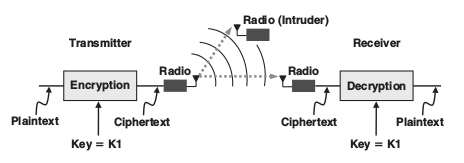
\includegraphics[scale=0.5]{./img/img_zigbee_aes}}

Niezaszyfrowana wiadomość jest nazywana \textit{plaintext} czyli tekstem jawnym natomiast zaszyfrowana nosi w literaturze obcojęzycznej nazwę \textit{ciphertext} czyli kryptogram. Algorytmy szyfrujące do jakich zalicza się AES są typowo algorytmami blokowymi, ponieważ tekst jawny dzieli się na bloki które następnie są szyfrowane, również przy odszyfrowywaniu kryptogram jest dzielony na bloki które są odszyfrowywane za pomocą tajnego klucza. ZigBee używa 128 bitowych bloków szyfrujących/deszyfrujących. \\
AES jest algorymtem symetrycznym stąd szyfrowanie i deszyfrowanie jest realizowane za pomocą tego samego klucza który jest z założenia tajny i jedynie porozumiewające się strony mają do niego dostęp. Klucz szyfrujący jest w postaci binarnej i jest umieszczany w odpowiednich urządzeniach za pomocą różnych technik o których często decyduje producent układów lub konstruktor rozwiązania wykorzystującego WSN.
Zigbee wspiera klucze szyfrujące AES wielkości 128, 196 i 256bitów, oraz implementuje metody rozdzielania i utrzymywania tych kluczy w sieci. Pomimo faktu, że sieci standard dopuszcza jedynie możliwość symetrycznej kryptografii podczas transmisji są wykorzystywane w praktyce dwa symetryczne klucze: \textit{linked key} oraz \textit{network key}. \\
\textit{Linked key} jest kluczem dzielonym jedynie między dwoma węzłami i jest on wykorzystywany w pojedyńczej komunikacji.\\
\textit{Network key} natomiast jest współdzielony przez wszystkie urządzenia mające dostęp do sieci i jest wykorzystywany do samego procesu dołączenia do sieci, oraz komunikacji jeden do wielu (\textit{broadcasting}). \\ 
Sieć implementująca szyfrowanie wiadomości musi również posiadać urządzenie o specjalnym przeznaczeniu tzn. cenfrum zaufania (\textit{trust center}). Może nim być koordynator sieci ale również każde inne urządzenie warunek jest taki że jedna sieć ma jedno i tylko jedno centrum zaufania które służy do dystrybucji kluczy, i jego adres jest ustalany przez koordynatora sieci.

\paragraph{Trust center i mechanizmy zarządzania kluczami} 

\par W poprzednim paragrafie zostało wspomniane o dwóch kluczach występujących w sieciach ZigBee a mianowicie o dynamicznie przyznawanym \textit{Linked Key} oraz permanentnym przypisanym do sieci \textit{Network Key}. Istnieją trzy metody przypisywania klucza do urządzenia: preinstalacja (\textit{preinstallation}), transportowanie klucza (\textit{key transport}) oraz ustalenie klucza (\textit{key establishment}). \\
Preinstalacja polega na wbudowaniu klucza podczas procesu wytwarzania. Metoda ta często jest potocznie nazywana hardcodowaniem klucza i może odbywać się na różne sposoby np. generowanie klucza podczas procesu programowania urządzenia i zapisywanie go w pamięci nieulotnej, jak i również na umieszczaniu go w specjalnej sekcji na etapie samego wytwarzania krzemowego układu. Korzystając z takiego rozwiązania urządzenia przyłączające się do sieci nie potrzebują odpytywać \textit{trust center} o klucz sieciowy ponieważ już nim dysponują. W wielu aplikacjach preinstalacja jest najbardziej bezpieczną metodą rozprowadzania tajnego klucza sieciowego ponieważ jest on przekazywany jedynie na etapie produkcji który z założenia jest bezpieczny.\\
Metoda transportowania klucza polega na procesie odpytywania poprzez urządzenie przyłączone do sieci \textit{trustcenter} o klucz sieciowy. Całość zapytania odbywa się w warstwie APS, w której \textit{trustcenter} decyduje czy wysłać urządzeniu klucz sieciowy czy też nie. powyższasesja odbywa się za pomocą nieszyfrowanego połączenia, co oczywiście stanowi istotną lukę bezpieczeństwa uniemożliwiającą stosowanie tej metody w wielu krytycznych zastosowaniach. Rozwiązaniem tego problemu jest stosowanie tzw. \textit{key-transport key}. KTK używa dodatkowego klucza który jest wykorzystany do transmisji tajnego klucza. \\
Trzecią z metod jaką jest przypisywanie poprzez ustalenia klucza polega na stworzeniu losowego klucza między dwoma komunikującymi się ze sobą urządzeniami omijając nieszyfrowane bezprzewodowe kanały komunikacyjne. W sieciach WSN bazujących na protokole ZigBee protokół ustalania klucza korzysta z symetrycznego protokołu ustalania klucza (




